
\appendix

\section{Entrada balística i sustentadora a la Terra}

A continuació es presentaran les gràfiques calculades amb el mateix format que l'article de John C. Adams, Jr. \cite{adams} amb dues pàgines, cadascuna amb 11 plots. La primera amb l'entrada balística i la segona amb l'entrada sustentadora.

També s'han realitzat distincions amb els coeficients balístics i els angles inicials. Les $\beta$ s'han mantingut amb unitats imperials per a que es pugui visualitzar ràpidament amb valors enters. Es important recalcar que com els càlculs s'han realitzat en SI, això ja s'ha tingut en compte mitjançant factors de conversió en la programació.
% Escribir aquí un texto bonito que justifique why dejamos media pagin en blanco y luego hay 2 paginas con 11 plots cada una
% Cambiar tambien el titulo

\begin{figure}[ht]
    \centering
    \begin{subfigure}[t]{.33\textwidth}
        \centering
        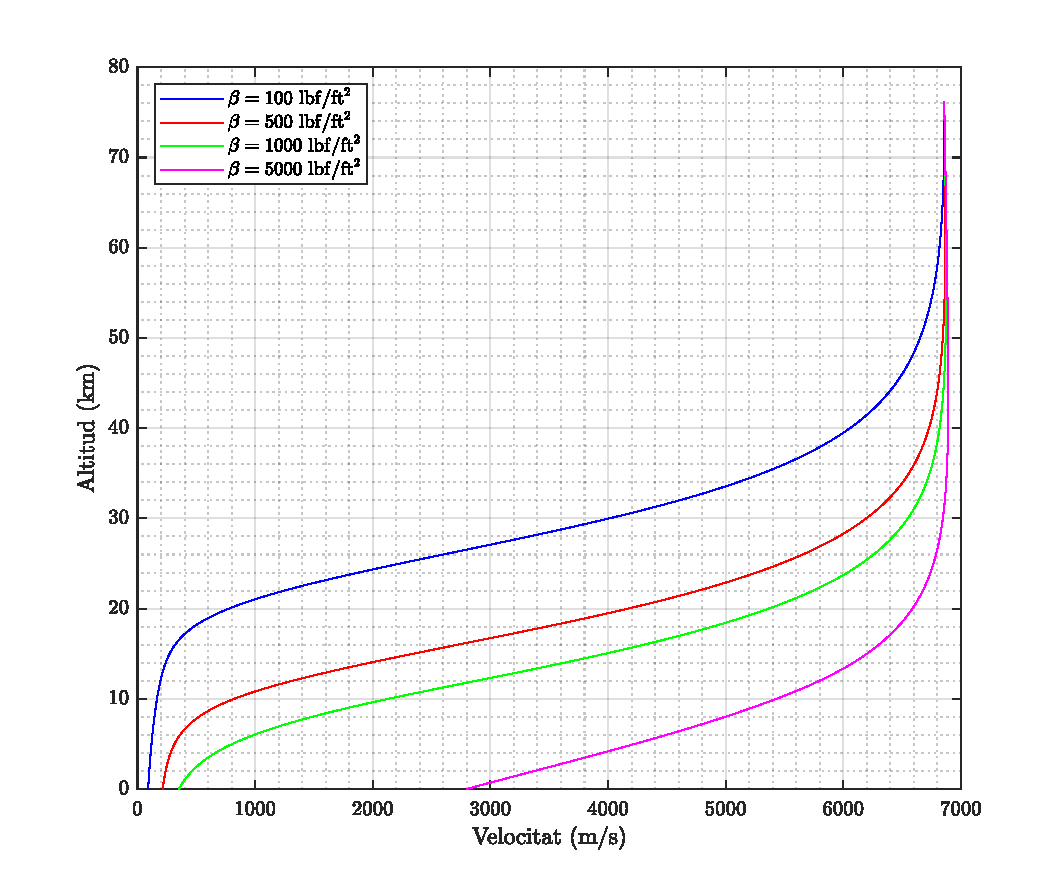
\includegraphics[width=\linewidth]{imagenes/01_ballistic_graficas/velocitat_no_title.pdf}
        \captionsetup{skip=0pt}
        \caption{Velocitat ($\meter/\second$)}
    \end{subfigure}%
    \begin{subfigure}[t]{.33\textwidth}
        \centering
        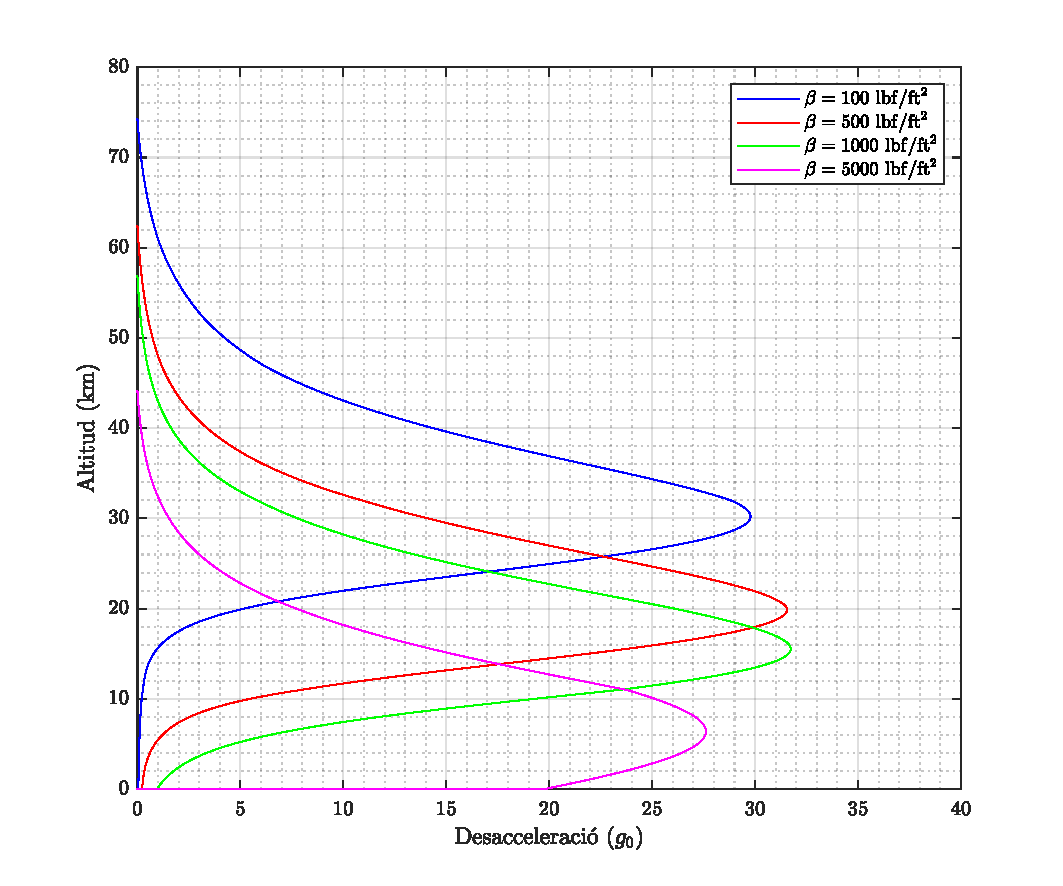
\includegraphics[width=\linewidth]{imagenes/01_ballistic_graficas/desacceleracio_no_title.pdf}
        \captionsetup{skip=0pt}
        \caption{Desacceleració ($g$)}
    \end{subfigure}%
    \begin{subfigure}[t]{.33\textwidth}
        \centering
        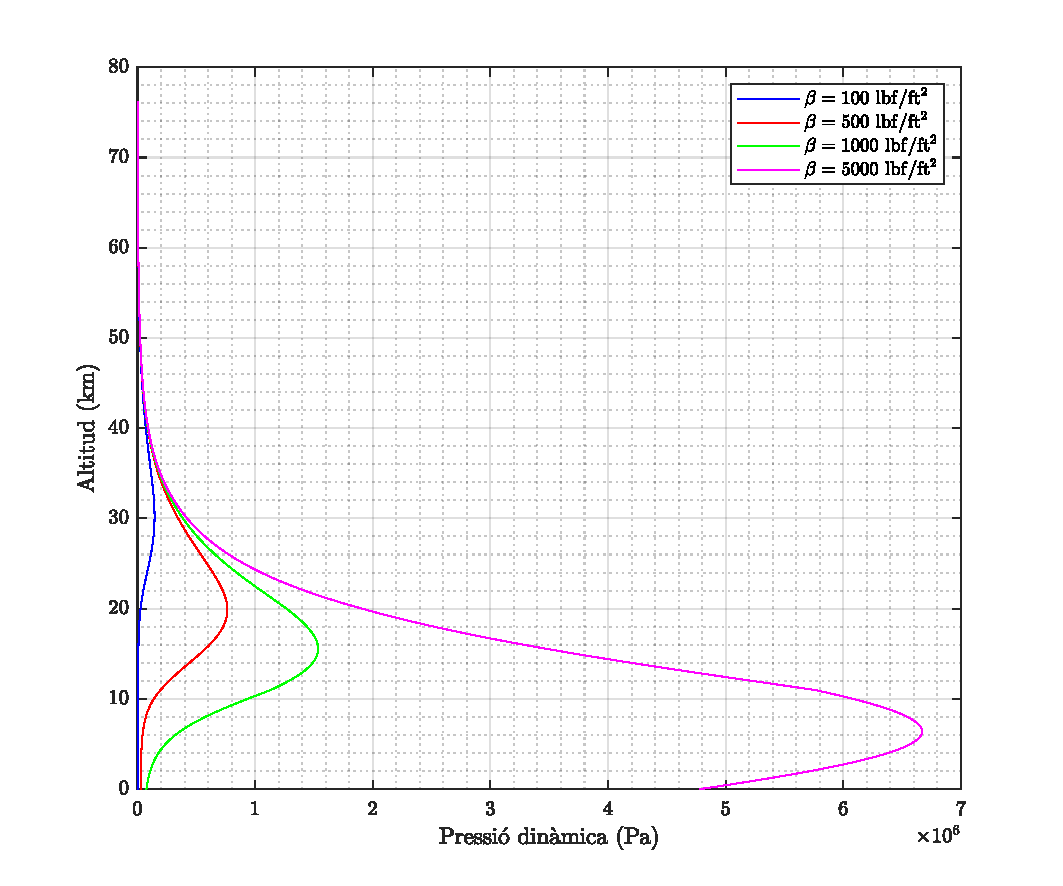
\includegraphics[width=\linewidth]{imagenes/01_ballistic_graficas/pressio_dinamica_no_title.pdf}
        \captionsetup{skip=0pt}
        \caption{Pressió dinàmica ($Pa$)}
    \end{subfigure}
    % Siguiente línea
        \begin{subfigure}[t]{.33\textwidth}
        \centering
        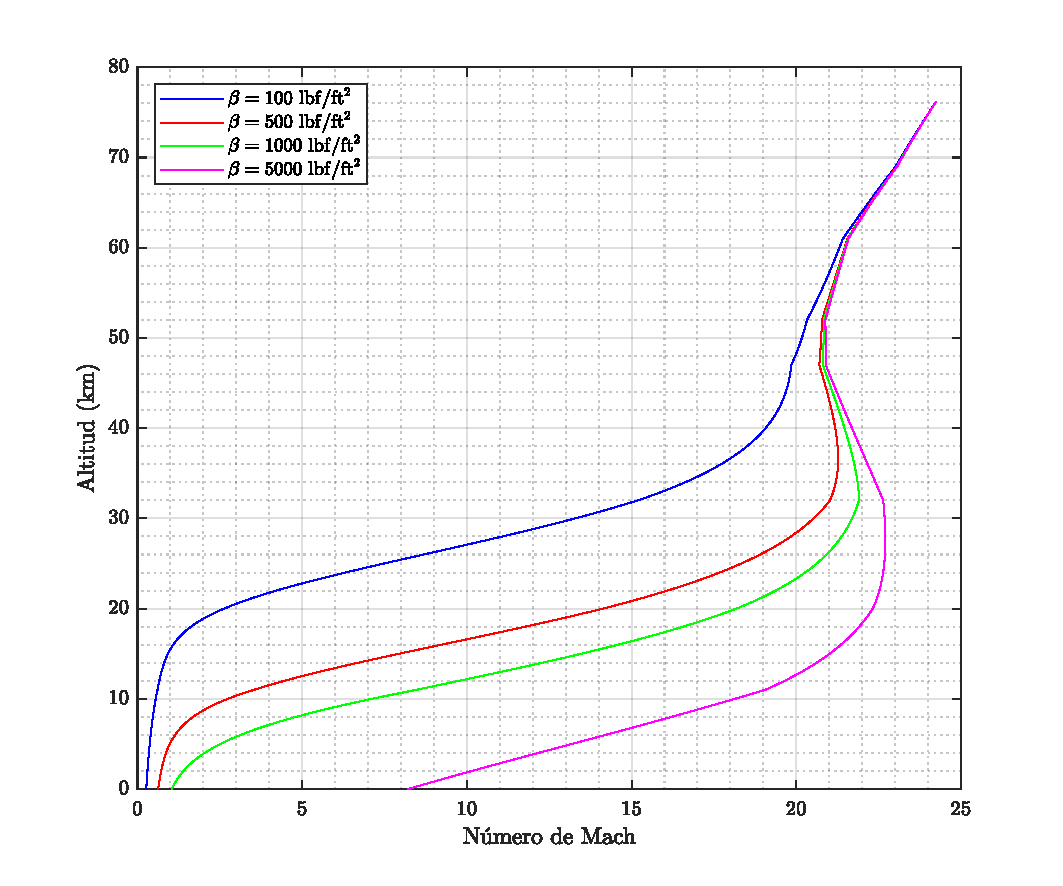
\includegraphics[width=\linewidth]{imagenes/01_ballistic_graficas/mach_no_title.pdf}
        \captionsetup{skip=0pt}
        \caption{Número de Mach ($\mathrm{adim}$)}
    \end{subfigure}%
    \begin{subfigure}[t]{.33\textwidth}
        \centering
        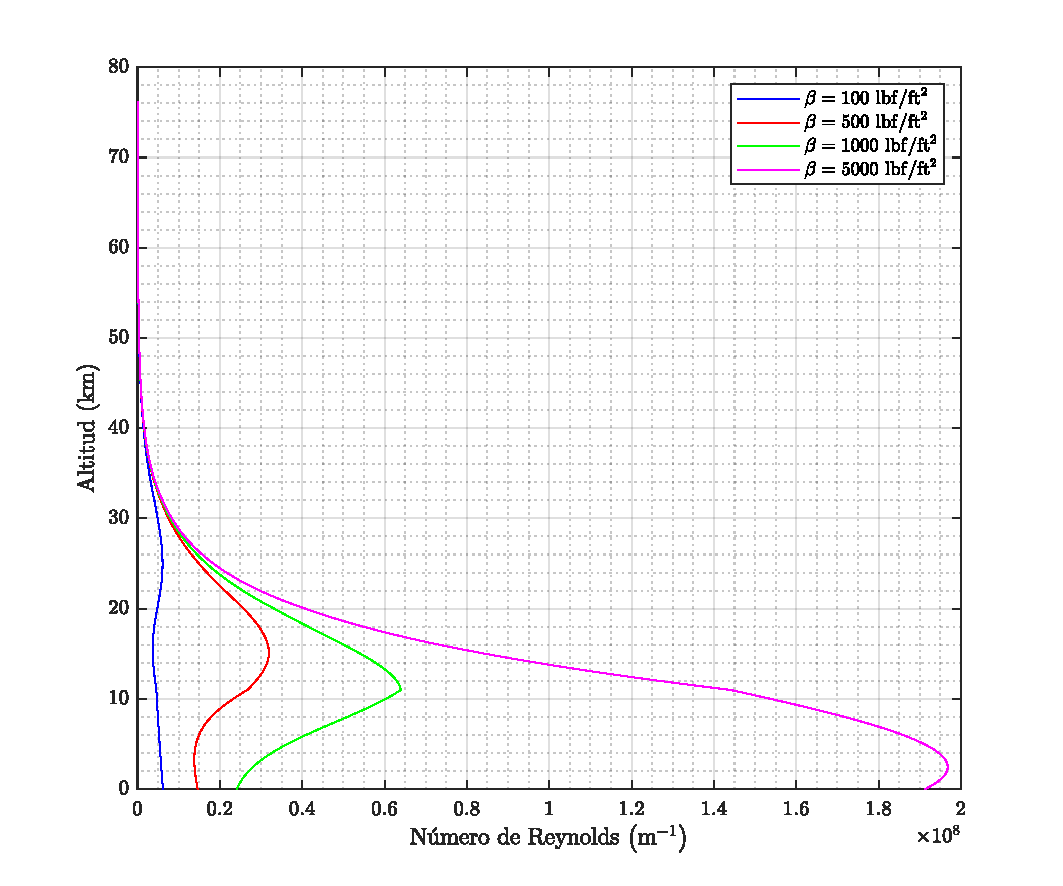
\includegraphics[width=\linewidth]{imagenes/01_ballistic_graficas/reynolds_no_title.pdf}
        \captionsetup{skip=0pt}
        \caption{Número de Reynolds ($\mathrm{adim}$)}
    \end{subfigure}%
    \begin{subfigure}[t]{.33\textwidth}
        \centering
        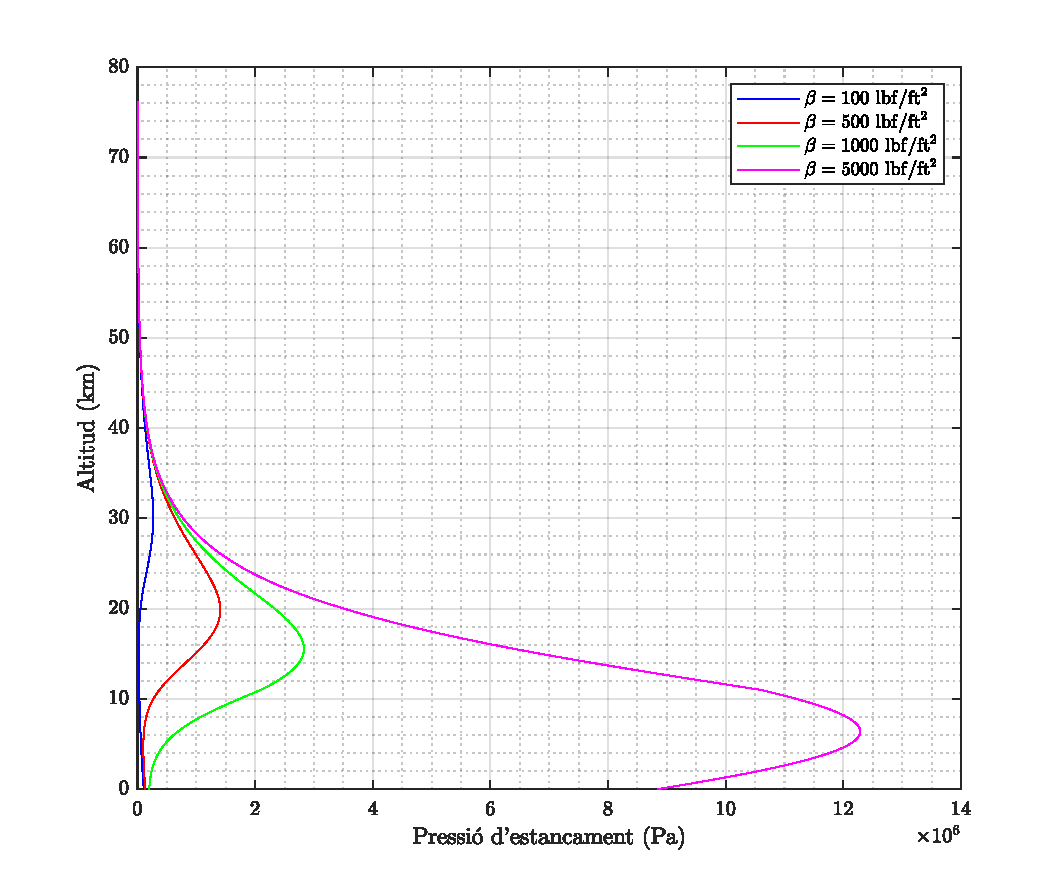
\includegraphics[width=\linewidth]{imagenes/01_ballistic_graficas/pressio_estancament_no_title.pdf}
        \captionsetup{skip=0pt}
        \caption{Pressió d'estancament ($\pascal$)}
    \end{subfigure}
    % Siguiente línea
        \begin{subfigure}[t]{.33\textwidth}
        \centering
        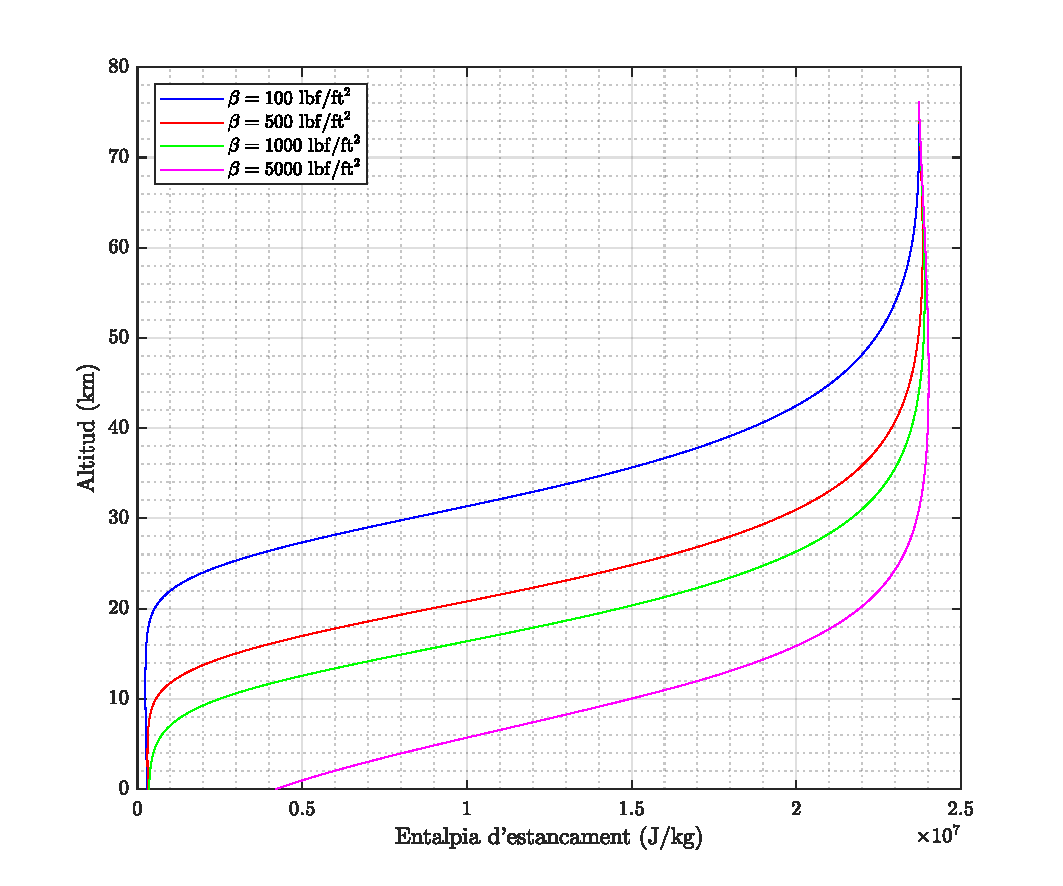
\includegraphics[width=\linewidth]{imagenes/01_ballistic_graficas/entalpia_estancament_no_title.pdf}
        \captionsetup{skip=0pt}
        \caption{Entalpia estancament ($\joule / \kilo\gram$)}
    \end{subfigure}%
    \begin{subfigure}[t]{.33\textwidth}
        \centering
        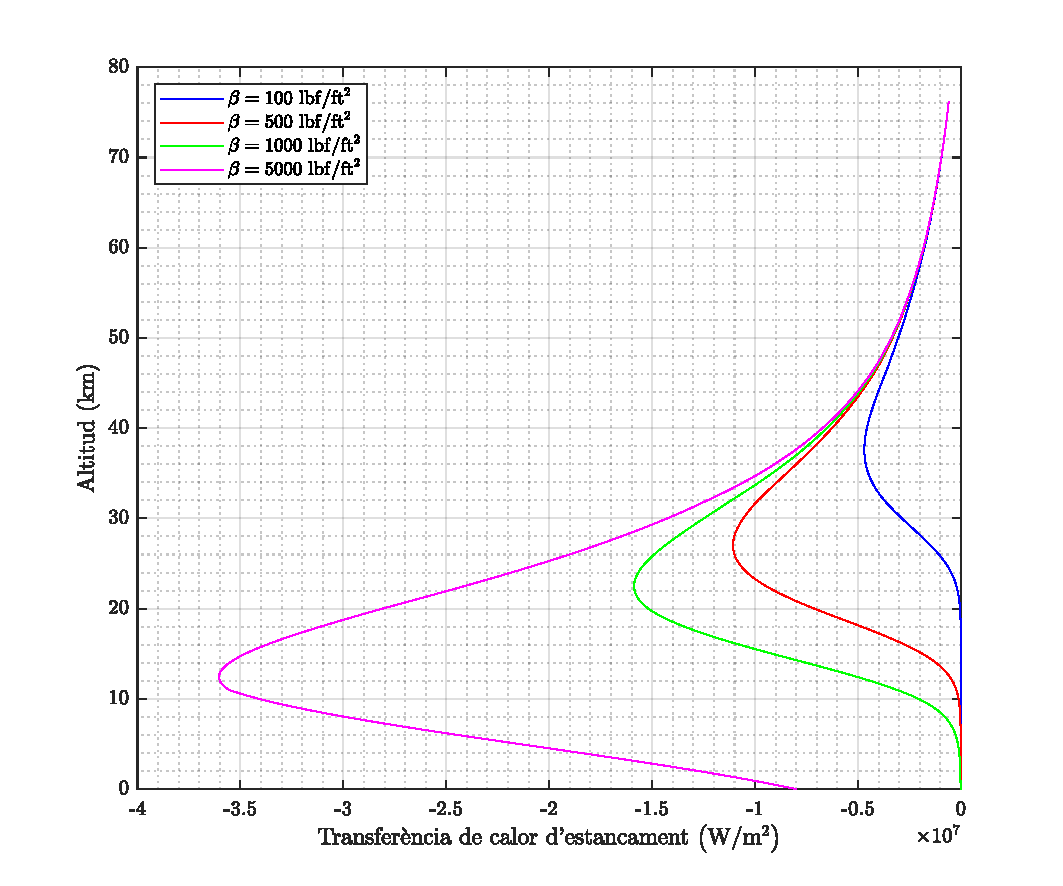
\includegraphics[width=\linewidth]{imagenes/01_ballistic_graficas/transferencia_calor_estancament_no_title.pdf}
        \captionsetup{skip=0pt}
        \caption{Transferència calor estancament ($\joule/\meter^2\second$)}
    \end{subfigure}%
    \begin{subfigure}[t]{.33\textwidth}
        \centering
        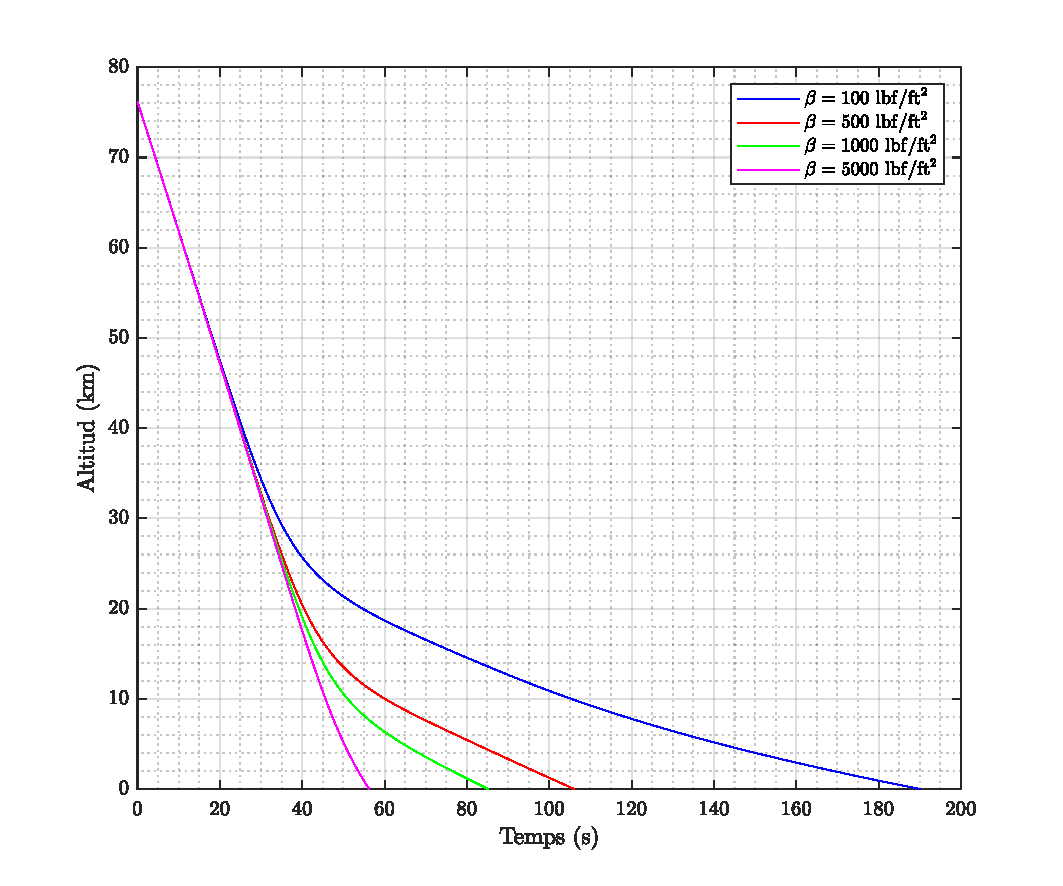
\includegraphics[width=\linewidth]{imagenes/01_ballistic_graficas/temps_no_title.pdf}
        \captionsetup{skip=0pt}
        \caption{Temps de reentrada ($\second$)}
    \end{subfigure}
    % Siguiente línea
        \begin{subfigure}[t]{.33\textwidth}
        \centering
        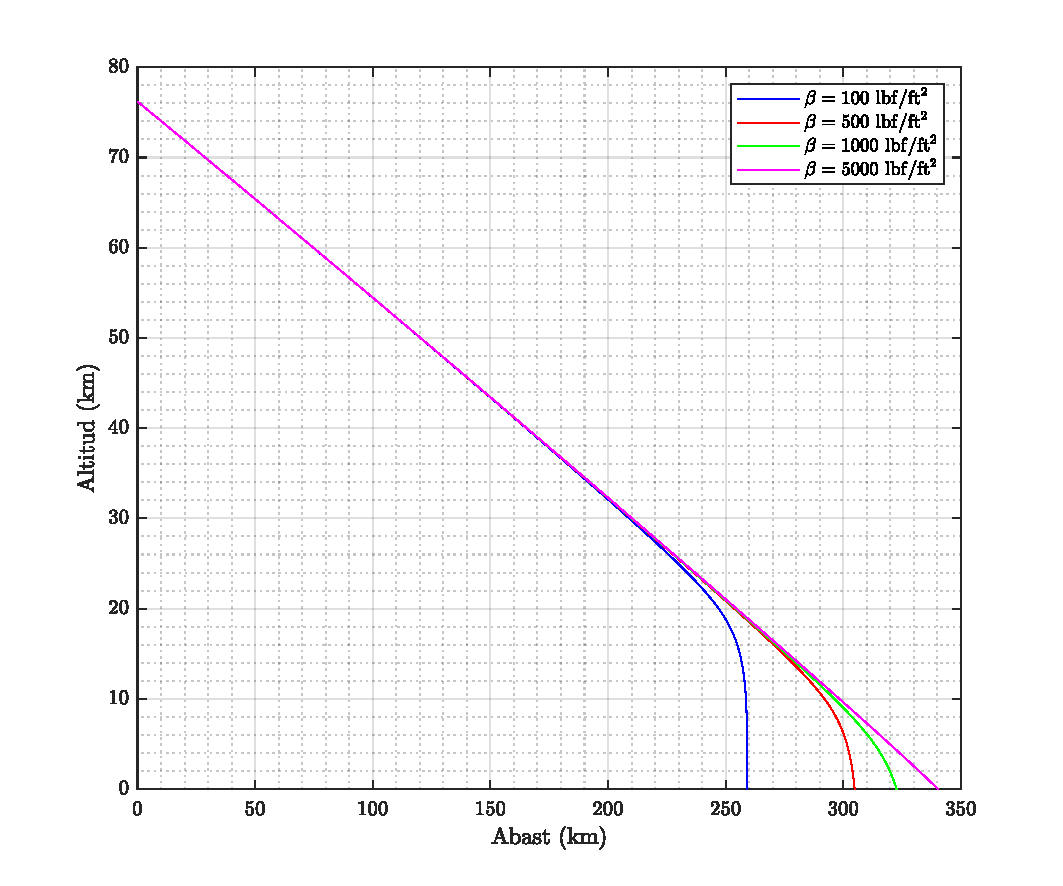
\includegraphics[width=\linewidth]{imagenes/01_ballistic_graficas/abast_no_title.pdf}
        \captionsetup{skip=0pt}
        \caption{Abast ($\meter$)}
    \end{subfigure}%
    \begin{subfigure}[t]{.33\textwidth}
        \centering
        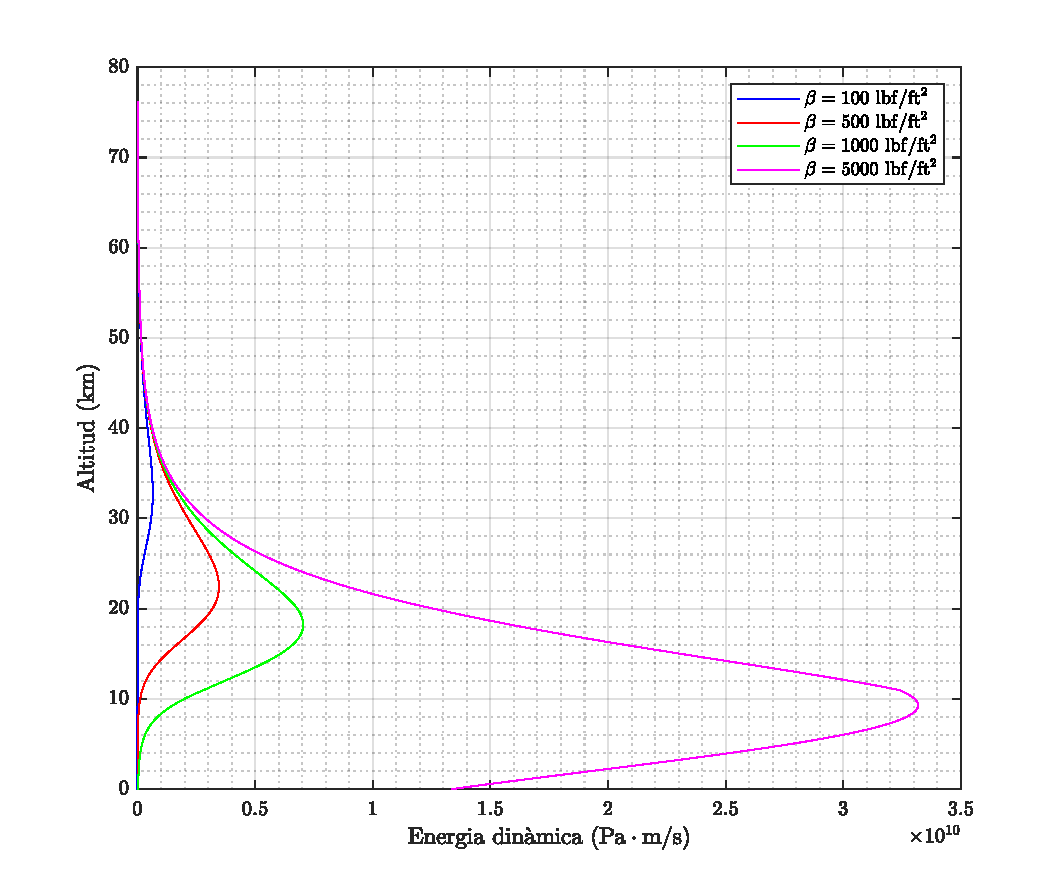
\includegraphics[width=\linewidth]{imagenes/01_ballistic_graficas/energia_dinamica_no_title.pdf}
        \captionsetup{skip=0pt}
        \caption{Energia dinàmica ($\pascal \cdot \meter/\second$)}
    \end{subfigure}
    \caption{Trajectòria de reentrada balística a la Terra}
    \label{fig:ballistic_terrestre}
\end{figure}

\begin{figure}[ht]
    \centering
    \begin{subfigure}[t]{.33\textwidth}
        \centering
        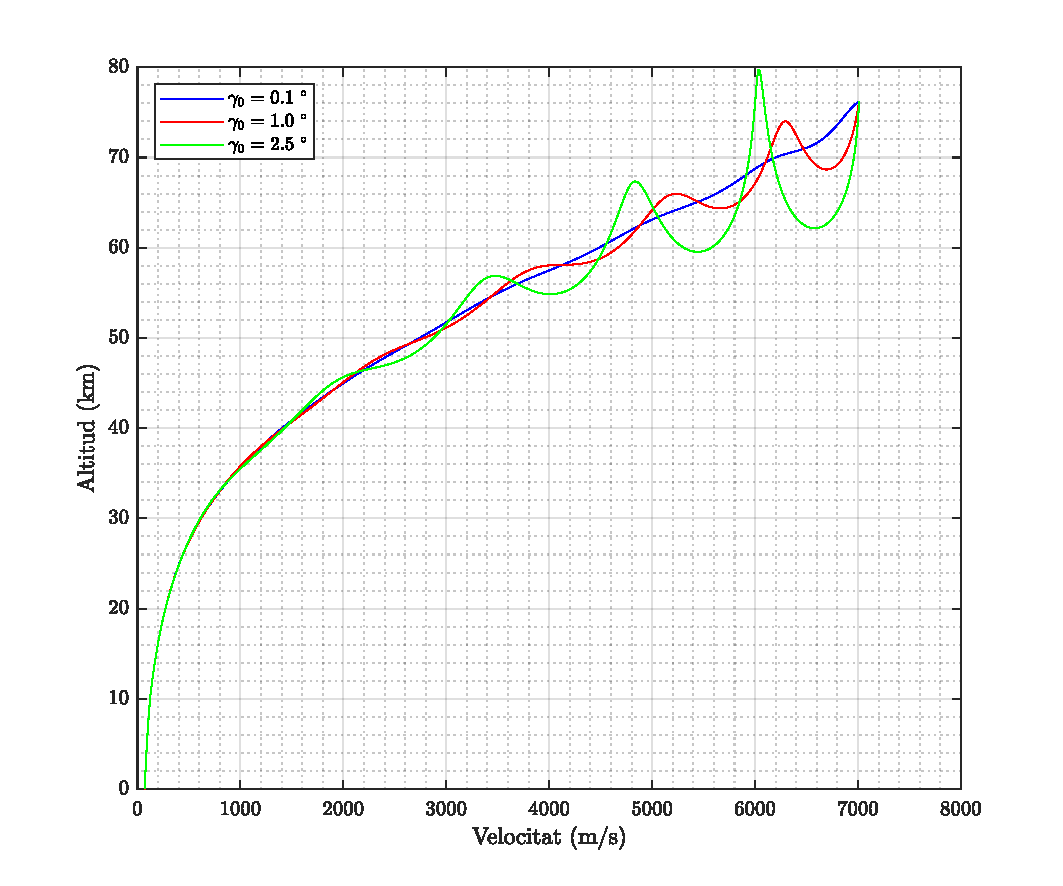
\includegraphics[width=\linewidth]{imagenes/02_lifting_graficas/velocitat_no_title.pdf}
        \caption{Velocitat ($\meter/\second$)}
    \end{subfigure}%
    \begin{subfigure}[t]{.33\textwidth}
        \centering
        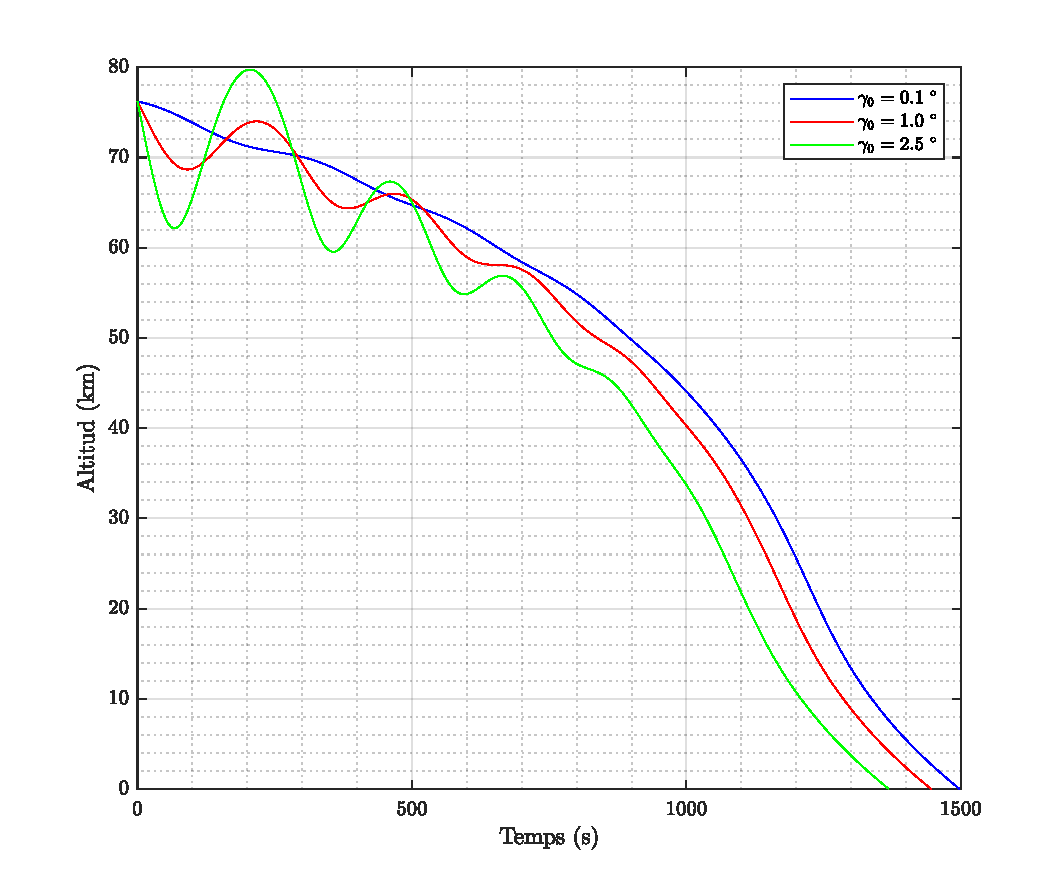
\includegraphics[width=\linewidth]{imagenes/02_lifting_graficas/temps_no_title.pdf}
        \caption{Temps de reentrada ($\second$)}
    \end{subfigure}%
    \begin{subfigure}[t]{.33\textwidth}
        \centering
        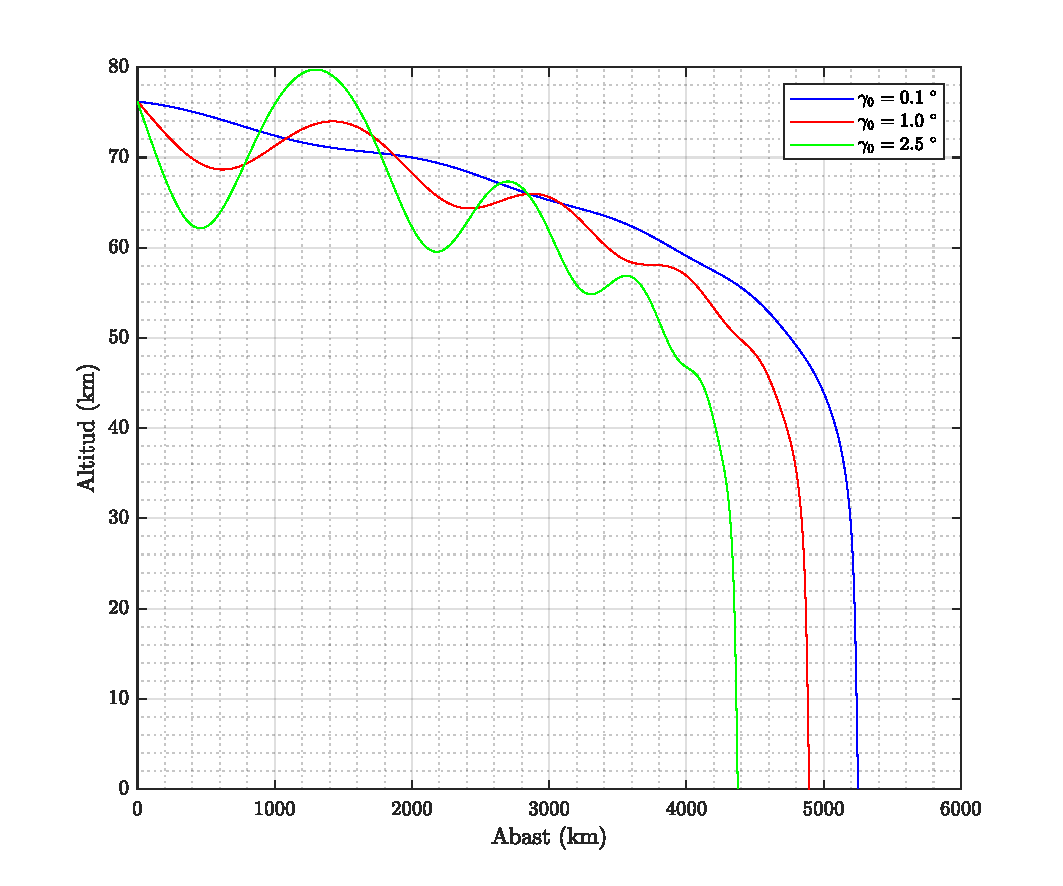
\includegraphics[width=\linewidth]{imagenes/02_lifting_graficas/abast_no_title.pdf}
        \caption{Abast ($\meter$)}
    \end{subfigure}
    % Siguiente línea
        \begin{subfigure}[t]{.33\textwidth}
        \centering
        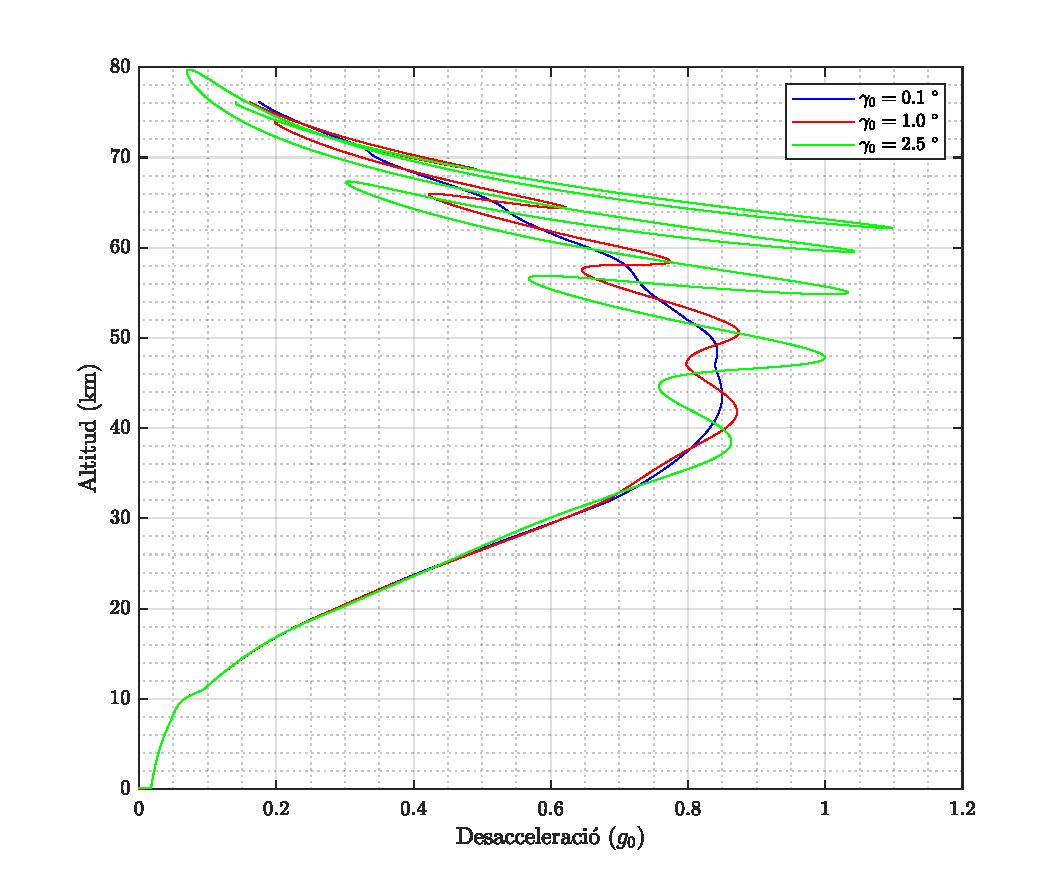
\includegraphics[width=\linewidth]{imagenes/02_lifting_graficas/desacceleracio_no_title.pdf}
        \caption{Desacceleració ($g$)}
    \end{subfigure}%
    \begin{subfigure}[t]{.33\textwidth}
        \centering
        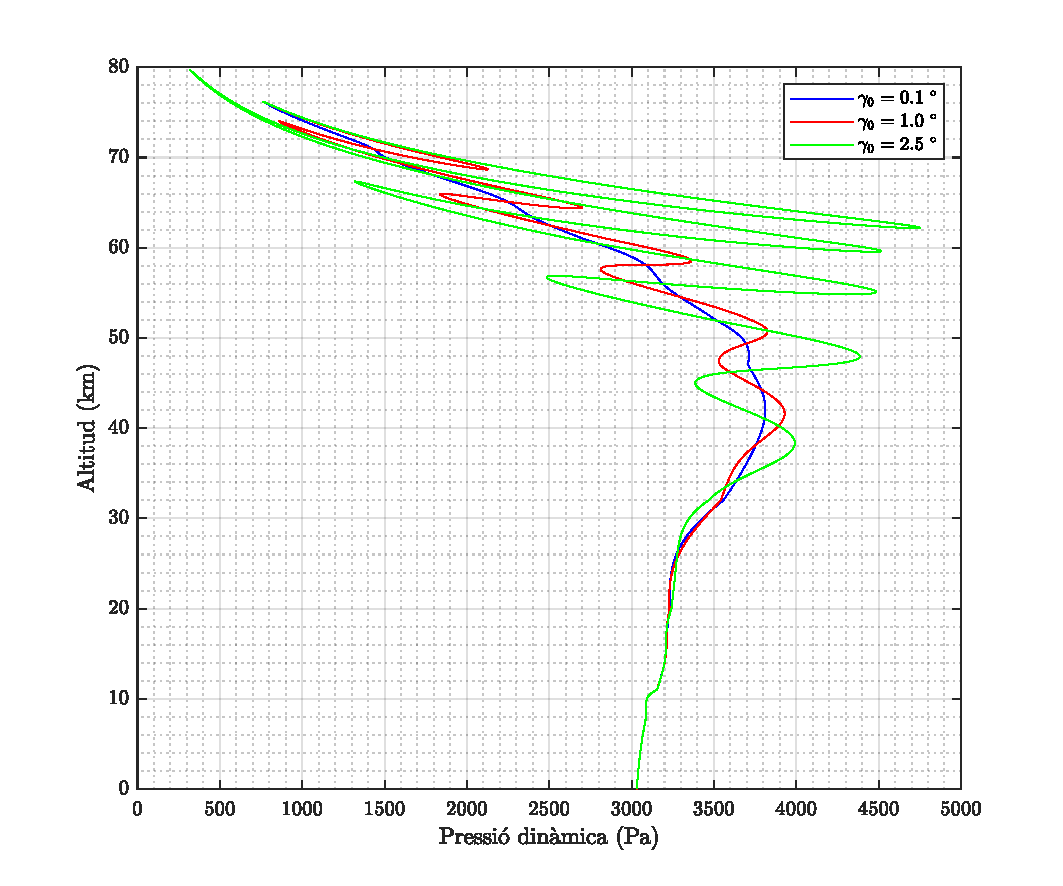
\includegraphics[width=\linewidth]{imagenes/02_lifting_graficas/pressio_dinamica_no_title.pdf}
        \caption{Pressió dinàmica ($Pa$)}
    \end{subfigure}%
    \begin{subfigure}[t]{.33\textwidth}
        \centering
        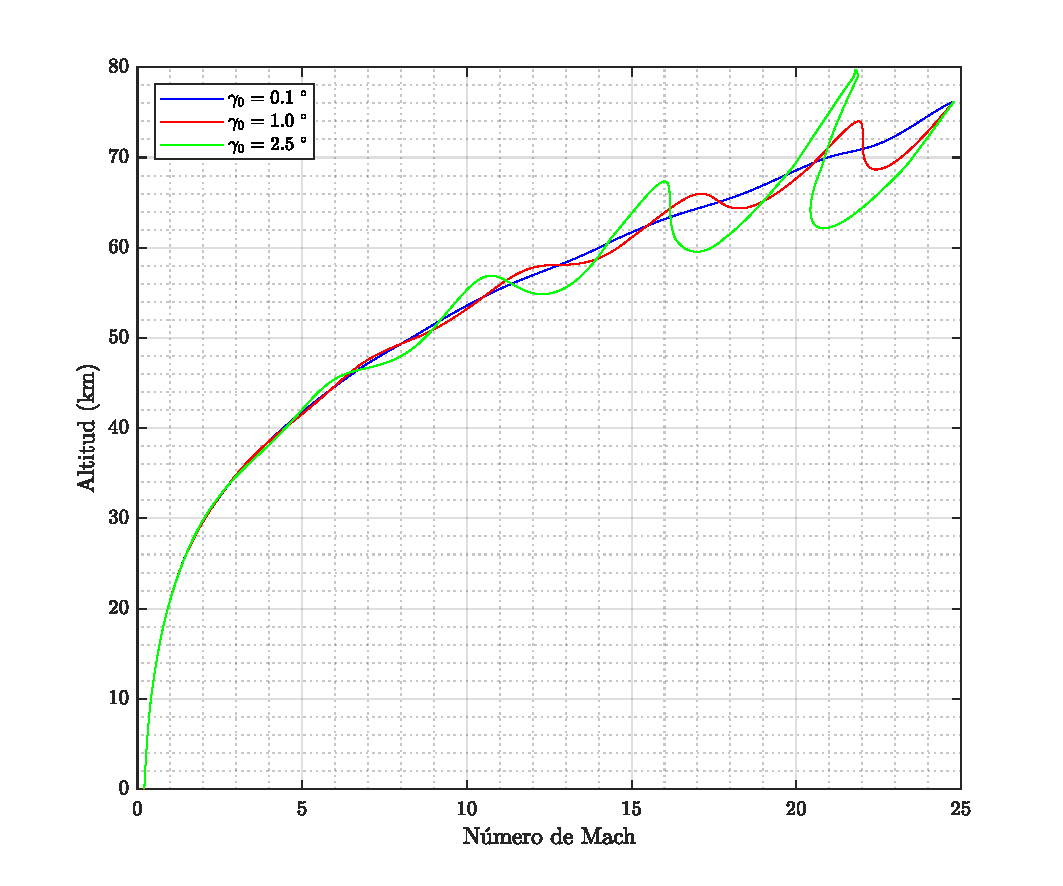
\includegraphics[width=\linewidth]{imagenes/02_lifting_graficas/mach_no_title.pdf}
        \caption{Número de Mach ($\mathrm{adim}$)}
    \end{subfigure}
    % Siguiente línea
        \begin{subfigure}[t]{.33\textwidth}
        \centering
        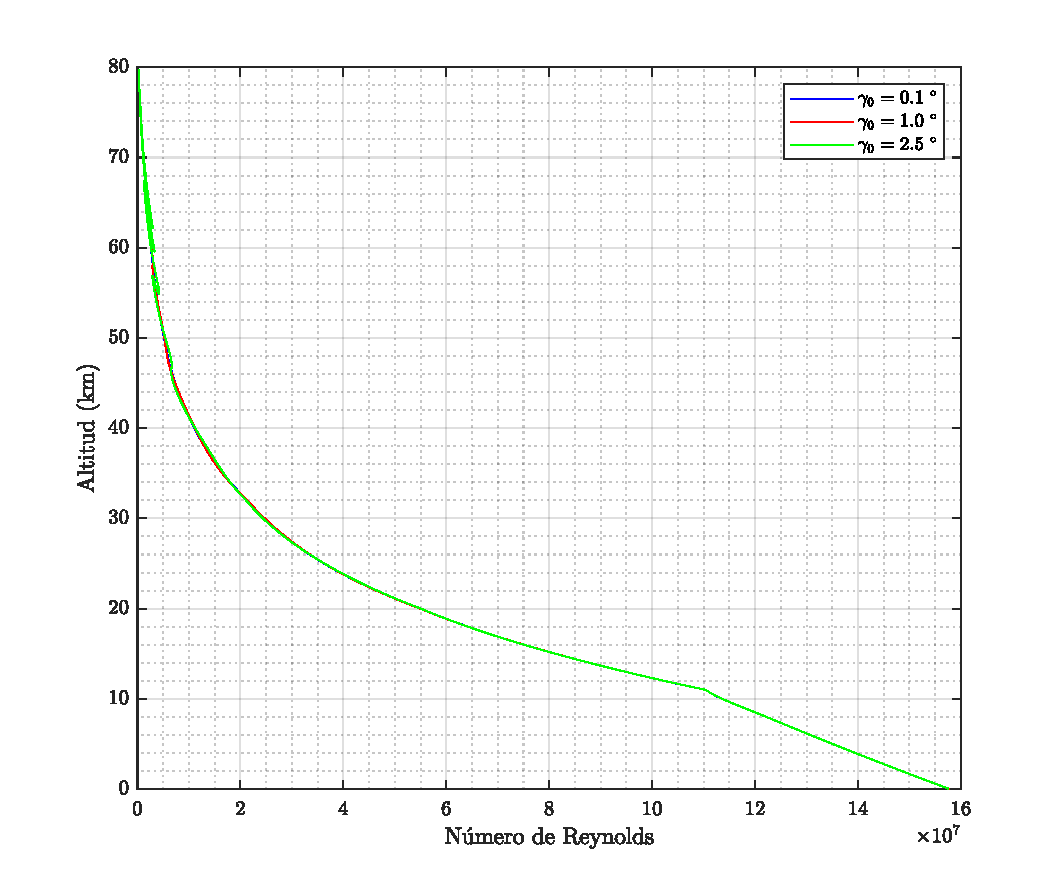
\includegraphics[width=\linewidth]{imagenes/02_lifting_graficas/reynolds_no_title.pdf}
        \caption{Número de Reynolds ($\mathrm{adim}$)}
    \end{subfigure}%
    \begin{subfigure}[t]{.33\textwidth}
        \centering
        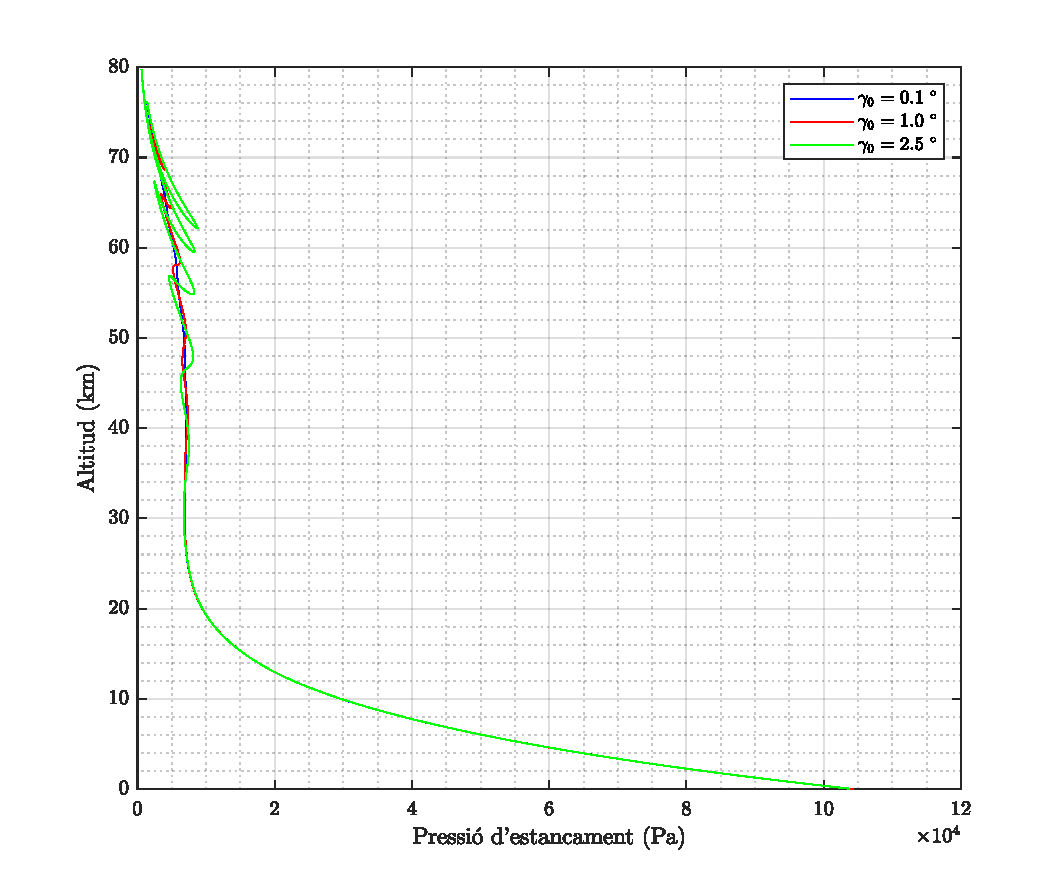
\includegraphics[width=\linewidth]{imagenes/02_lifting_graficas/pressio_estancament_no_title.pdf}
        \caption{Pressió d'estancament ($\pascal$)}
    \end{subfigure}%
    \begin{subfigure}[t]{.33\textwidth}
        \centering
        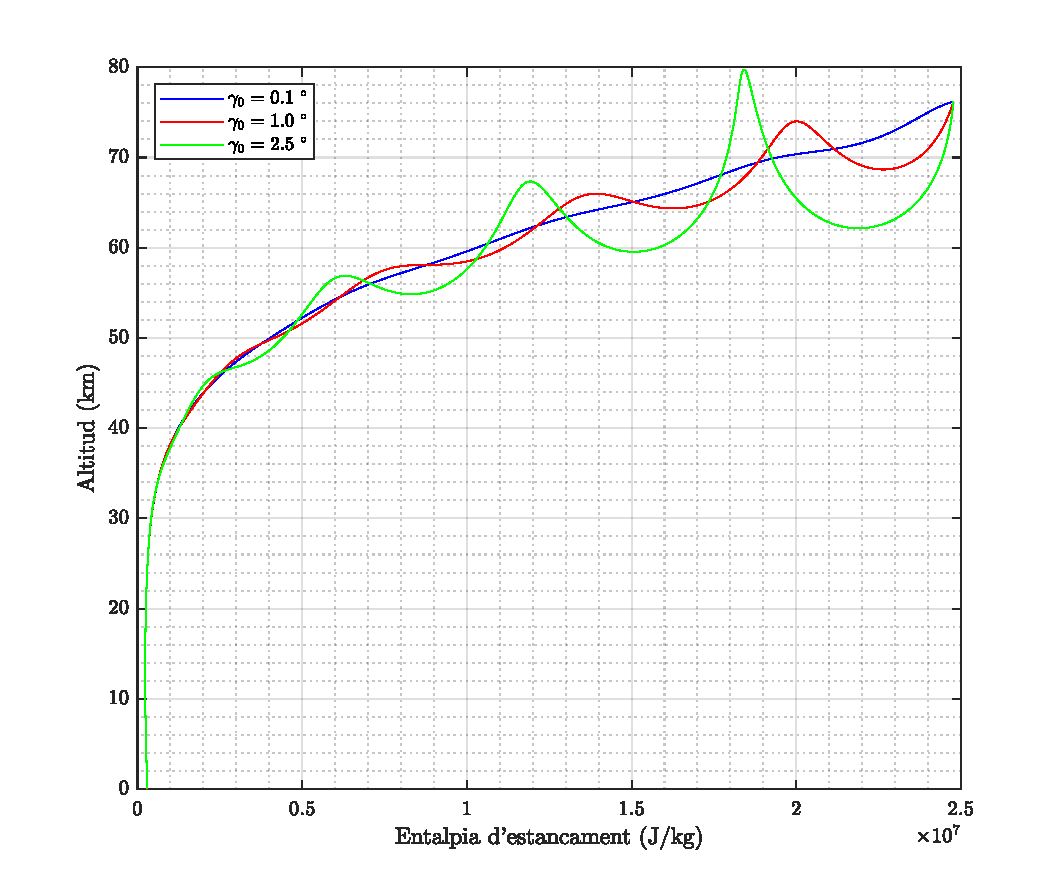
\includegraphics[width=\linewidth]{imagenes/02_lifting_graficas/entalpia_estancament_no_title.pdf}
         \caption{Entalpia d'estancament ($\joule / \kilo\gram$)}
    \end{subfigure}
    % Siguiente línea
        \begin{subfigure}[t]{.33\textwidth}
        \centering
        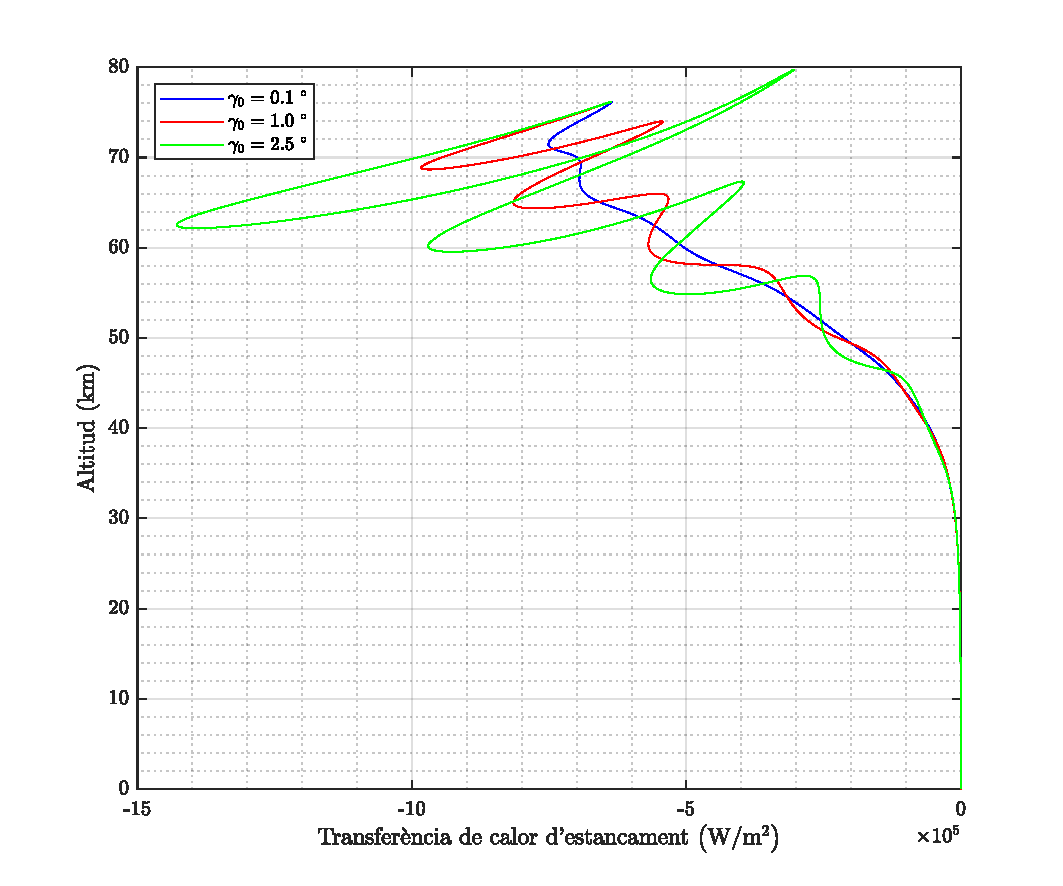
\includegraphics[width=\linewidth]{imagenes/02_lifting_graficas/transferencia_calor_estancament_no_title.pdf}
        \caption{Transferència de calor d'estancament ($\joule/\meter^2\second$)}
    \end{subfigure}%
    \begin{subfigure}[t]{.33\textwidth}
        \centering
        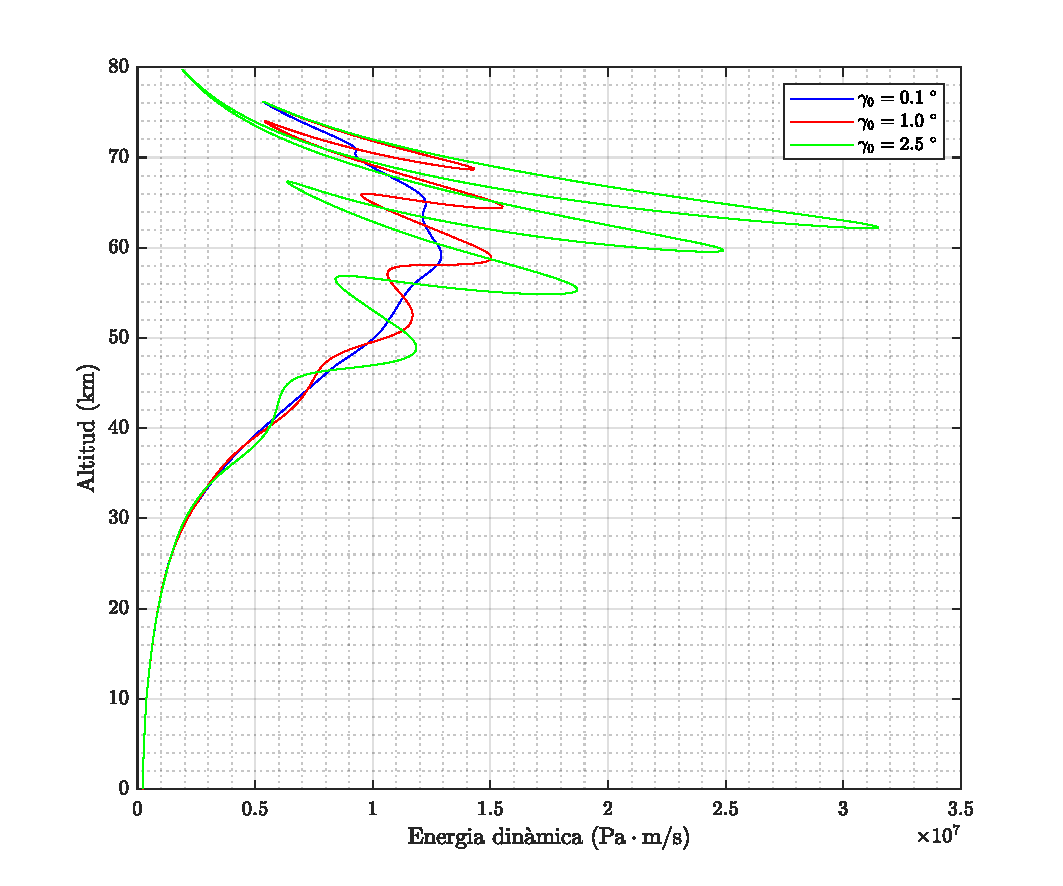
\includegraphics[width=\linewidth]{imagenes/02_lifting_graficas/energia_dinamica_no_title.pdf}
        \caption{Energia dinàmica ($\pascal \cdot \meter/\second$)}
    \end{subfigure}
    \caption{Trajectòria de reentrada sustentadora de l'Space Shuttle}
    \label{fig:lifting_terrestre}
\end{figure}

